\documentclass[11pt]{article}
\usepackage{amsmath,amsfonts,amssymb,eucal,graphicx}
\usepackage{epsfig}
%\usepackage{pslatex}
\usepackage{wrapfig}
\usepackage{exscale}
\usepackage{setspace}
\usepackage{subfigure}
\usepackage{color}
\usepackage{url} 
\usepackage{float}
\restylefloat{table}
\usepackage{enumitem}
\usepackage{titlesec}
\titleformat*{\section}{\large\bfseries}
\titleformat*{\subsection}{\normalsize\bfseries}
\titleformat*{\subsubsection}{\large\bfseries}
\titleformat*{\paragraph}{\large\bfseries}
\titleformat*{\subparagraph}{\large\bfseries}
\usepackage[font=footnotesize]{caption}
\usepackage[letterpaper, margin=1in]{geometry}
%\usepackage{showframe}
\usepackage{booktabs}
\usepackage{cite}

\hyphenation{test-bed}

\textwidth  6.6in
\textheight 9.1in
\setlength{\oddsidemargin}{-0.04 in}
\setlength{\topmargin}{-0.7in}
\newcommand{\alex}[1]{\textcolor{cyan}{ #1}}
\newcommand{\noi}{\noindent}
\newcommand{\bi}{\begin{itemize}}
\newcommand{\ei}{\end{itemize}}
\newcommand{\bc}{\begin{center}}
\newcommand{\ec}{\end{center}}

\newcommand{\toc}{{\em IEEE Trans.~Communications, }}
\newcommand{\tit}{{\em IEEE Trans.~Information Theory, }}
\newcommand{\jsac}{{\em IEEE J. Selected Areas Commun., }}
\newcommand{\rtime}[1]{\par\noindent\rlap{#1} \hspace*{2.15cm}}
\newcommand{\iblank}{\par \noindent \hspace*{2.4cm} \hangindent 2.6cm}

\newcommand{\nm}[1]{\textcolor{red}{\textbf{[NM: #1]}}}
\newcommand{\ca}[1]{\textcolor{blue}{\textbf{[CA: #1]}}}
\newcommand{\as}[1]{\textcolor{cyan}{\textbf{[AS: #1]}}}

\def\etal{{\em et al.\/}}
\def\eg{{\em {\em e.g.},\ }}
\def\ie{{\em i.e.,\ }}
\def\etc{{\em etc.\ }}
\def\be{\begin{equation}}
\def\ee{\end{equation}}

\newcommand{\SNR}{{\sf SNR}}
\newcommand{\INR}{{\sf INR}}
\newcommand{\SINR}{{\sf SINR}}
\newcommand{\Nc}{{\cal N}}
\newcommand{\Ec}{{\cal E}}
 
 \newfont{\bb}{msbm10 scaled 1100}
\newcommand{\CC}{\mbox{\bb C}}
\newcommand{\PP}{\mbox{\bb P}}
\newcommand{\RR}{\mbox{\bb R}}
\newcommand{\QQ}{\mbox{\bb Q}}
\newcommand{\ZZ}{\mbox{\bb Z}}
\newcommand{\FF}{\mbox{\bb F}}
\newcommand{\GG}{\mbox{\bb G}}
\newcommand{\EE}{\mbox{\bb E}}
\newcommand{\NN}{\mbox{\bb N}}
\newcommand{\KK}{\mbox{\bb K}}

%\renewcommand{\baselinestretch}{0.965}

\begin{document}

\begin{center}
\textbf{\Large Adaptive Wireless Networks for Spectrally Efficient Communication} \\[0.1in]
\Large DARPA SC2: Phase 2 Technical Paper \\
Team BAM!\ Wireless
\end{center}

\tableofcontents
\newpage

\listoffigures
\newpage
\section{Summary}
A description of the key technical aspects of the design of the BAM! Wireless Collaborative Intelligent Radio Network (CIRN) that was developed in Phase 2 of the DARPA SC2 Challenge is provided in this paper. The presented design adapts intelligently to the existing Colosseum scenario as well as the behavior of peer teams, in a robust manner that takes into account a wide range of error or unexpected event possibilities. As illustrated in the sequel, reaching this solution required innovating lightweight intelligent capabilities on top of flexible and robust physical and network layers.

\section{Introduction}
We present in this paper important aspects of the technical design of the BAM!\ Wireless Collaborative Intelligent Radio Network (CIRN) that participated in the second preliminary event of DARPA SC2. The CIRN consists of multiple Standard Radio Nodes (SRN) and one Gateway node, as depicted in Figure~\ref{fig:high-level}. All nodes interact directly with the Colosseum emulator, while only the gateway can send and receive collaboration messages according to the defined CIRN Interaction Language (CIL). 

 
\begin{figure} [htb]
 \centerline{
 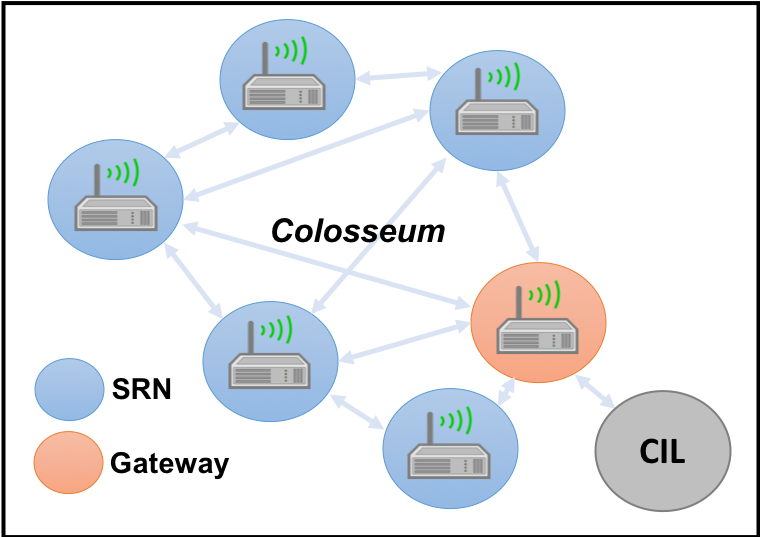
\includegraphics[width = 0.6\textwidth]{Figures/SysBD.png}}
 \caption{BAM!\ Wireless Network for the DARPA SC2 \cite[Figure $1$]{func-report}.} 
 \label{fig:high-level}
 \end{figure} 
 
Following the Phase 2 scoring procedure, the approach behind the BAM!\ Wireless CIRN design is centrally focused on maximizing the minimum number of achieved mandates by a team in any given match (ensemble minimum), by regularly monitoring the reported performance and use of resources of peer teams through the received collaboration messages. The CIRN design specifically relies on lightweight intelligent algorithms that are robust to changing environmental conditions. The final outcome is a robust intelligent solution that jointly optimizes the decisions for the modulation and coding scheme, flow scheduling, as well as channel allocation to maximize the ensemble performance in the wide range of Colosseum scenarios\footnote{A brief introduction to the BAM!\ Wireless team and solution is also available at https://www.spectrumcollaborationchallenge.com/teams/bam-wireless/}. We next describe in detail the various technical components of the CIRN.
 
\section{Methods, Assumptions, and Procedures}
We describe in this section the different components and tasks involved in the CIRN, and where each task is taking place across the layer architecture. We provide a high-level description in Figure~\ref{fig:arch}. Note that the \emph{Network Controller} function pertain only to the Gateway node; all other components and features  are common to all SRN nodes as well as the Gateway. We first start by describing the physical layer protocol below.
\begin{figure} [htb]
 \centerline{
 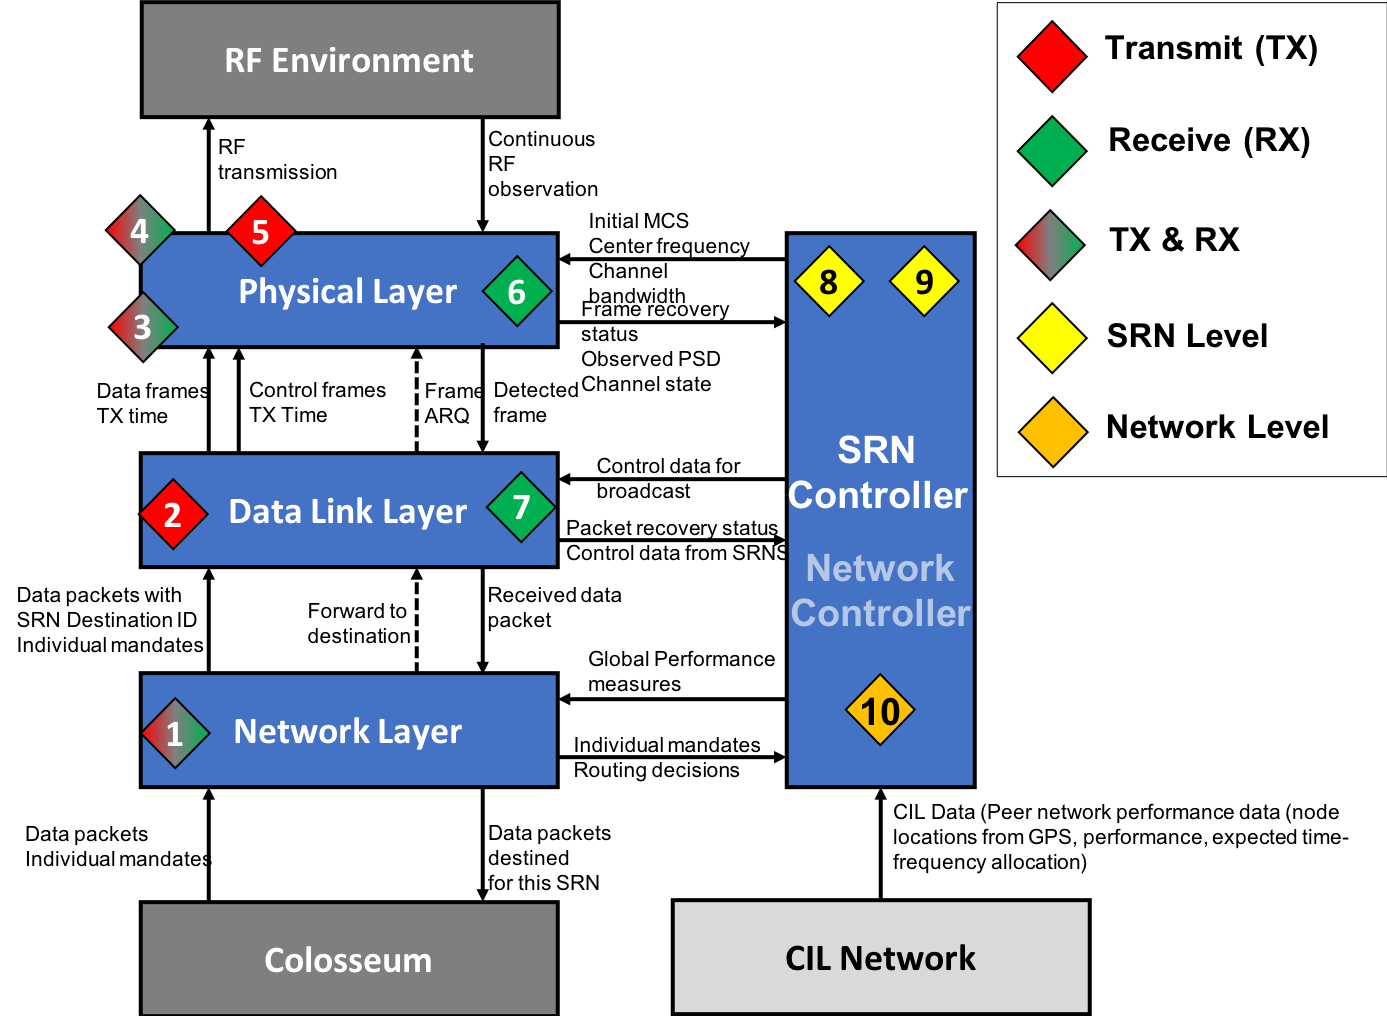
\includegraphics[width = 0.9\textwidth]{Figures/SysFuncBD.png}}
 \caption{High-level diagram showing the different layers and functional components of the BAM!\ Wireless CIRN \cite[Figure $2$]{func-report}. The numbered features in diamonds are: 1- Multi-Hop Routing, 2-Transmit Scheduling, 3-Broadcast of Control Data, 4-High Rate Data Link, 5-Transmit Power Control, 6-Adaptive Modulation and Coding Scheme, 7-Automatic Repeat Request, 8- Program Configuration through Database, 9- Visualization of Performance Measures, 10- Channel Allocation Algorithm.}
 \label{fig:arch}
 \end{figure} 
\subsection{Physical Layer Protocol}
As described in \cite{func-report}, we use a DFT-s-OFDM waveform with different choices for the bandwidth, center frequency, and power spectrum (see Figure \ref{fig:physical}). Each channel is defined by a choice of a center frequency and bandwidth pair, and each SRN is assigned a channel for transmission at any given point in time. Further, each SRN can listen to all other nodes in the network through multiple \emph{receive chains}. Each waveform occupies 108 subcarriers for data symbols, 12 subcarriers for pilot symbols, and 8 subcarriers that are used for estimating the noise variance. An algorithm similar to Schmidl \& Cox time synchronization is used by all receivers. The used modulation types are QPSK, 16-QAM, 32-QAM, and 64-QAM. The error correction codes are selected from the IEEE 802.11 QC-LDPC suite of codes with rates 1/2, 2/3, 3/4, and 5/6.  
\begin{figure} [htb]
     \centerline{
     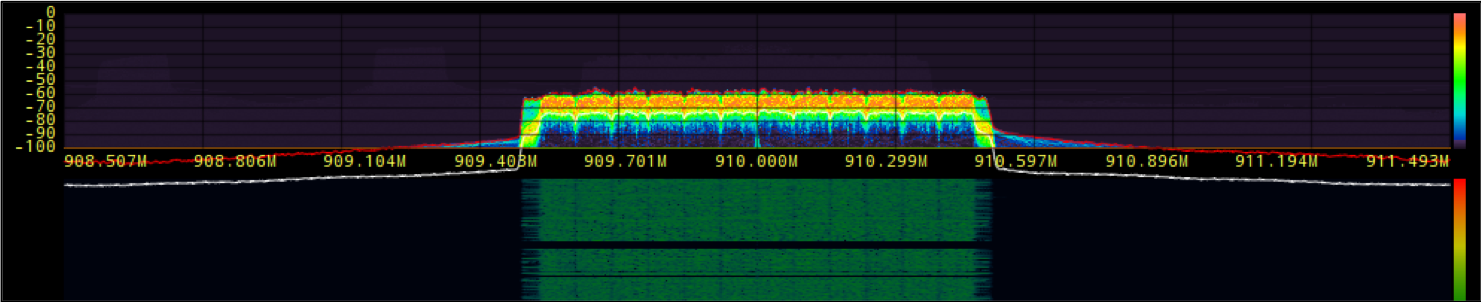
\includegraphics[width = 0.8\textwidth]{Figures/PowSpec.png}}
     \caption{Power spectrum of employed waveform \cite[Figure $6$]{func-report}.}
     \label{fig:physical}
     \end{figure}
In Figure~\ref{fig:ber}, we plot the simulated block error rates for different choices of the modulation scheme and code rate at a wide range of SNR values. 
\begin{figure} [htb]
     \centerline{
     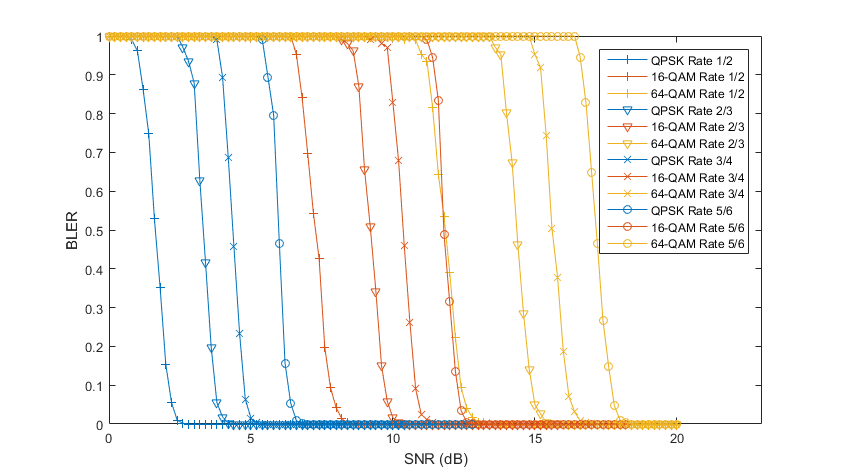
\includegraphics[width = 0.6\textwidth]{Figures/BLER.png}}
     \caption{Block error rates at different SNR levels for all combinations of supported pairs of modulation scheme and code rate \cite[Figure $7$]{func-report}.}
     \label{fig:ber}
     \end{figure}

\subsubsection{Frame Header}
We use QPSK modulation and a rate 1/2 code for frame headers. A frame header includes the source and destination identifiers, the modulation and coding scheme index, and the number of blocks carried in the frame payload.  Frame headers also include latency critical control and feedback information; currently ARQ feedback is included. To further minimize the probability of not correctly identifying the frame header, an extra protection is provided using a 32-bit cyclic redundancy code. Finally, the header also contains a frame identification number, which is used for data logging and analysis.

\subsubsection{Frame Payload}
A pair of modulation scheme and coding rate is selected for the frame payload based on the current environment, as described below. The blocks within the frame payload are mapped to subcarriers of a sequence of OFDM symbols. The content of a block originate from segments, which can be either IPv4 segments carrying Colosseum data,  segments carrying automatic repeat request information, or control segments.

\subsubsection{Adaptive MCS Scheme}
The employed adaptive MCS scheme is based on finding the smallest Euclidean distance between the boundaries of circles centered around constellation symbols. Each of these circles has a radius that is proportional to the ratio of estimated \emph{noise+interference} standard deviation and asymptotic code gain. The following factors are further considered:
\begin{enumerate}
    \item A lower bound on throughput is respected.
    \item An upper bound on block error rate is respected.
\end{enumerate}
For the second constraint above, a closed form approximation is assumed for computing the block error rate given the minimum distance between constellation points and noise standard deviation. 

Note that the noise variance estimate relies on a sliding window median filter to remove outliers. In Figure \ref{fig:adaptivemcs}, we show an example for the illustrated adaptive MCS scheme on a Colosseum payline scenario. It is important to highlight that the link rate reduces as the measured standard deviation of the additive noise increases.
\begin{figure} [htb]
     \centerline{
     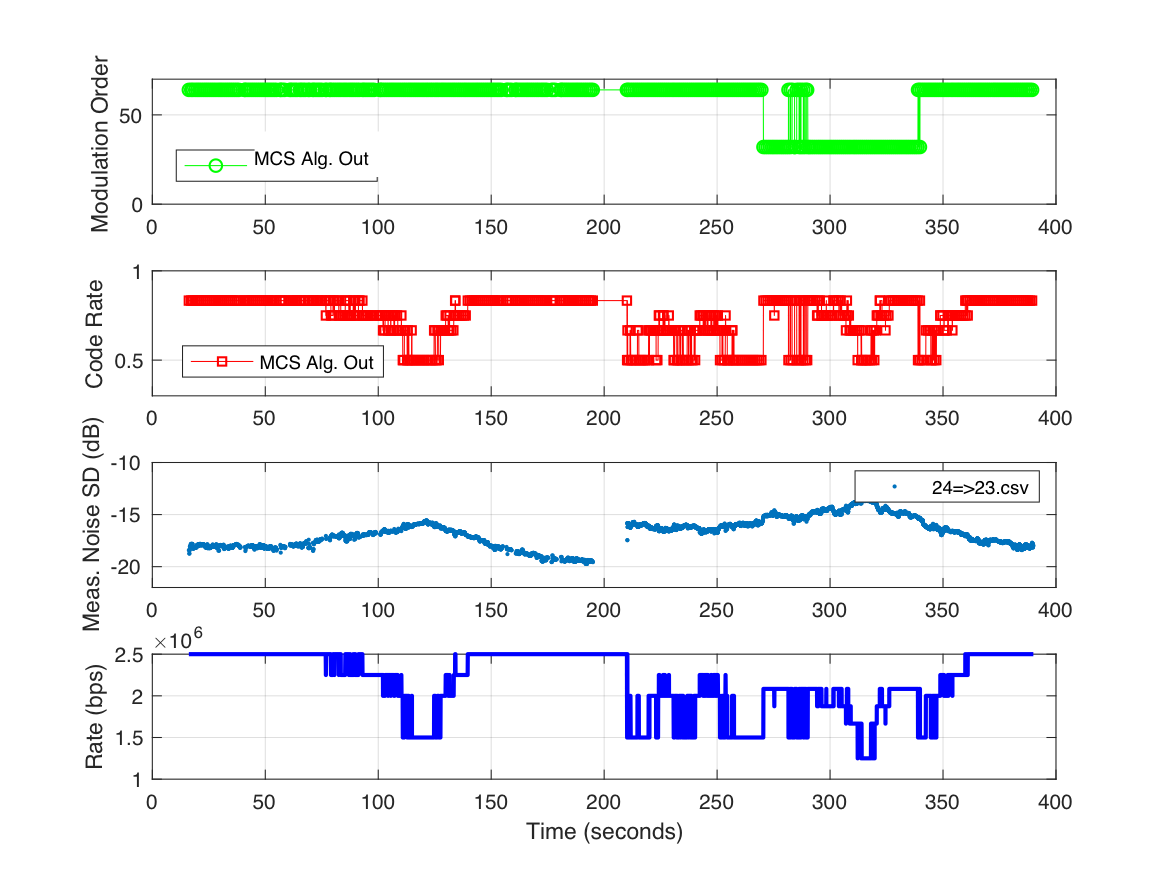
\includegraphics[width = 0.8\textwidth]{Figures/MCS.png}}
     \caption{Adaptation of modulation order and code rate due to change in estimated noise variance \cite[Figure $8$]{func-report}.}
     \label{fig:adaptivemcs}
     \end{figure}
\subsubsection{Transmit Power}
Our system uses one of the antennas for the data channel and the other for the control channel. Each transmission can only use half of the total power available to the radio. By default, we always transmit at maximum power. We only reduce our transmit power when we need to protect incumbents. This is done as follows.

A node-based transmit power control is employed for passive incumbent protection. Each incumbent regularly broadcasts a CIL message that contains it current channel information, measured total receive power, and a receive power threshold. When the measured power violates the threshold, the CIRN nodes should collectively lower transmit power levels, such that the violation ceases to exist at the incumbent. On the other hand, when the threshold is not violated, nodes are allowed to increase their transmit power levels while collectively respecting the incumbent constraint. Here, collaborative CIL messages are crucial to determine the total number of nodes - over all participating CIRNs - that are causing interference at the incumbent receiver.

Assuming non-coherent power combining at the receiver of the incumbent, the transmit power level for each SRN that causes interference at the incumbent is lowered, by an amount proportional to the violated distance from the threshold, and assuming that other networks will follow a similar procedure to lower the transmit power levels of nodes interfering at the incumbent receiver.
\subsection{Network Layer and Routing}
Here, we describe the multi-hop routing and automatic repeat request capabilities supported by the network layer.
\subsubsection{Multi-Hop Routing}
We detect the absence of a link between a pair of nodes through the absence of fresh control information. A binary routing table is then constructed after each nodes shares its local connectivity information. Dijkstra's algorithm is then applied to the routing table, in order to find the shortest path between the source and destination of a flow.
\subsubsection{Automatic Repeat Request (ARQ)}
Reliable flow transports is provided by a basic automatic repeat request (ARQ) mechanism based on sequence acknowledgements and a sliding-time window. First, we evaluate the reliability requirements of each flow, and determine whether automatic repeat request is needed. ARQ is enabled for all file flows for the CIRN that participated in the second preliminary event. ARQ for stream flows did not perform to standards and was disabled for the preliminary event 2.



\subsection{Flow Scheduling}
As different flows have different rate and latency requirements, we employ an adaptive scheduling algorithm that assigns \emph{time quanta}, and applies a deficit round-robin scheduling algorithm. Time quanta are assigned, such that a flow is scheduled if there is a good chance that it meets requirements. The applied deficit round-robin flow scheduling mechanism ensures fairness of the assigned time quanta.  Moreover, prioritization and anti-starvation is incorporated into the round-robin mechanism (thus allowing deviations from traditional and incorporation of ARQ for flow queuing (see Figure~\ref{fig:schedule} for an illustration).
\begin{figure} [htb]
     \centerline{
     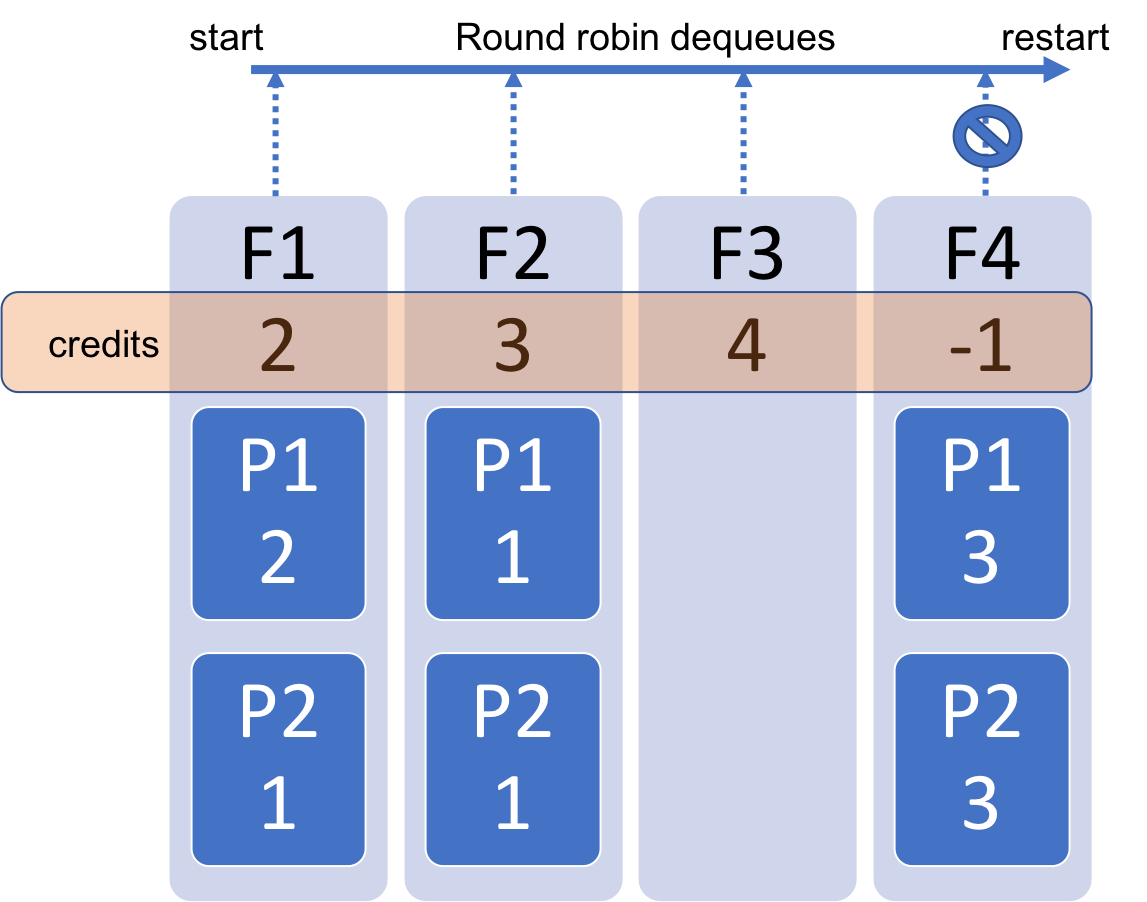
\includegraphics[width = 0.6\textwidth]{Figures/DeficitRR.png}}
     \caption{Example of deficit round-robin flow queue scheduling where flow queues $F\#$ with credits ($\#$) containing packets $P\#$ of size ($\#$) are scheduled \cite[Figure $3$]{func-report}.}
     \label{fig:schedule}
     \end{figure}
We envision a change in our flow scheduling algorithm based on the anticipated change in scoring in Phase 3. However, the structure of the adaptive algorithm need not change.     
\subsection{Control Channel}\label{sec:control}
We employ two types of control messages:
\begin{enumerate}
    \item Short control messages are transmitted with a modulation type of 8-FSK and a bandwidth of 480 KHZ. A time-hopping synchronization scheme is specially used for these control messages (see Figure \ref{fig:shortcontrol}). Also, a Reed-Solomon error control coding is used. The center frequency used for short control messages alternates every second between the upper and lower band edges\footnote{It is worth noting that we observed during the second preliminary event that this special allocation for short control messages caused problems when there is a badly performing peer team that is consistently requesting overlapping channels; we are investigating how to fix this issue for Phase 3.}.
    
    We use a variant of the Slotted ALOHA multiple access mechanism without collision detection and backoff, for short control messages. Every slot period is 60 ms. Nodes transmit short control messages at slot boundaries with a uniform probability whose value is inversely proportional to the number of nodes in the CIRN. The short control message carries information about the number of nodes in the network, the allocated channels, and a timestamp. Nodes broadcast modified states, upon receiving freshly updated short control messages. The advantage of having short control messages is to use it for initial node discovery, and as a reliable backup option when the interference level is high.
    
    \item Long control messages are carried within the DFT-s-OFDM data links. In addition to the basic information carried by short control messages, these long control messages carry information about traffic statistics and measured performance of individual mandates.
\end{enumerate}
\begin{figure} [htb]
     \centerline{
     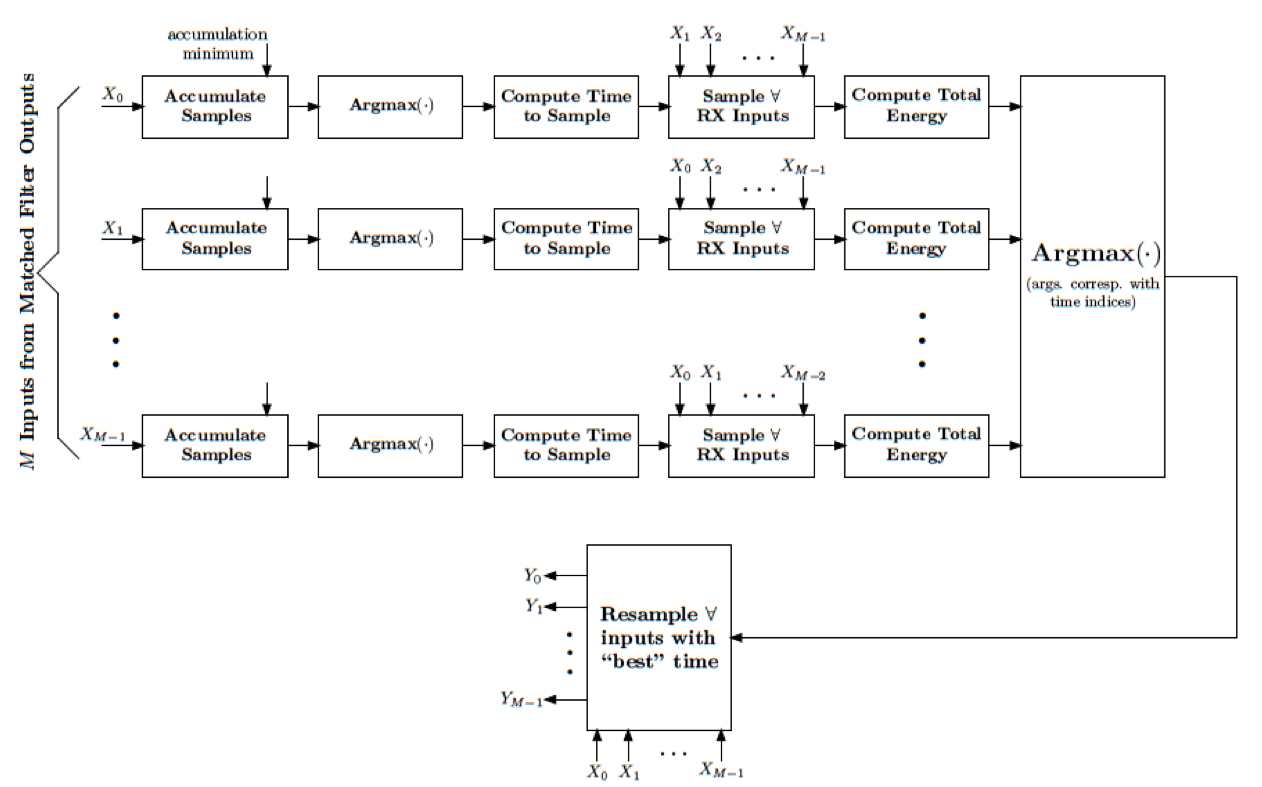
\includegraphics[width = 0.9\textwidth]{Figures/NDASync.png}}
     \caption{Robust synchronization method developed for the low signal-to-interference ratio scenario of the DARPA Spectrum Challenge leveraged for the BAM!\ wireless robust control link \cite[Figure $4$]{func-report}.}
     \label{fig:shortcontrol}
     \end{figure}
     
Figure~\ref{fig:controlband} shows the spectrogram that one of our nodes measured during a qualification scenario. Observe that short control messages occupy the narrow bands at the lower and upper edges. 

\begin{figure} [htb]
     \centerline{
     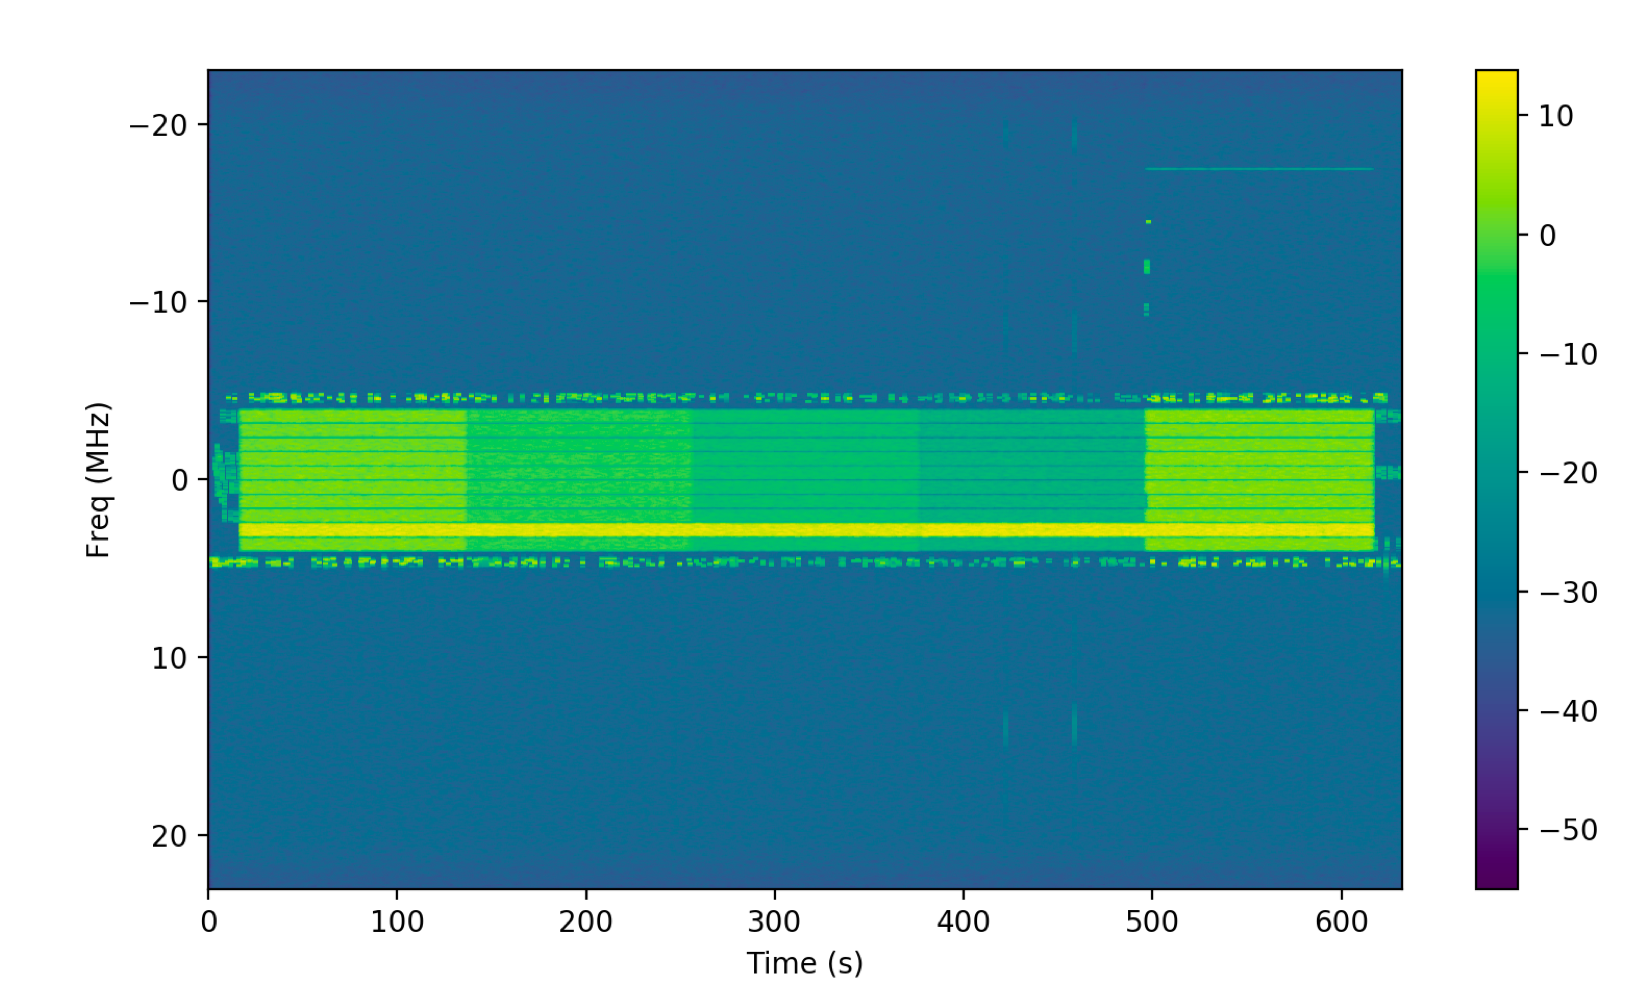
\includegraphics[width = 0.6\textwidth]{Figures/CCEx.png}}
     \caption{Control transmissions observed in SRN power spectrum \cite[Figure $5$]{func-report}.}
     \label{fig:controlband}
     \end{figure}
     
\subsection{Channel Allocation}
\label{s-chan_alloc}

The
gateway node first estimates the channel gain between our nodes and all others, using the GPS locations reported through the CIL and assuming free space propagation wtih loss exponent of 3. Our gain estimator assumes that gains frequency-independent, symmetric, and slowly varying. The channel gain is then refined adaptively by combining our own PSD measurements with other nodes' transmit power and frequency. The channel gain estimates and the spectrum voxel collaboration messages from other teams are
hence used to construct an interference map for each frequency. The interference spectrum is different
for each of our nodes, and varies across different frequencies. The gateway node goes through all the
frequency bands and determines individual interference levels for each of our nodes. Each node is then assigned a channels (center frequency and bandwith) to transmit on. This choice is made through a combination of a greedy algorithm that attempts to maximize our own score and a \emph{considerate} algorithm that reallocates channels to help improve the ensemble minimum. The channel allocation mechanism also responds to environmental updates and changes in offered mandates. If  a  node  needs  to  transmit  more  traffic  to  a  specific  receiver,  or  the  flows  have  more  stringent requirements, the gateway will take that into account when picking the center frequency.

It is important to highlight that an obstacle we faced towards making the channel allocation algorithm more biased towards a collaborative behavior was that the information that we were receiving from peer nodes (specifically, the GPS locations and SpectrumUsage) was frequently inaccurate.
 
In summary our nodes will receive on multiple channels, but transmit on a single one (apart from the control channel). The bandwidth required for each node is chosen based on the offered load. We plan to incorporate the new scoring mechanism of Phase 3 to bias the channel allocation mechanism towards a more greedy behavior in the stage where extra individual mandates contribute to score without regard to the ensemble.

We show in Figure~\ref{fig:channelalloc} example behavior of the channel allocation mechanism in an Alleys of Austin scenario.

\begin{figure} [htb]
     \centerline{
     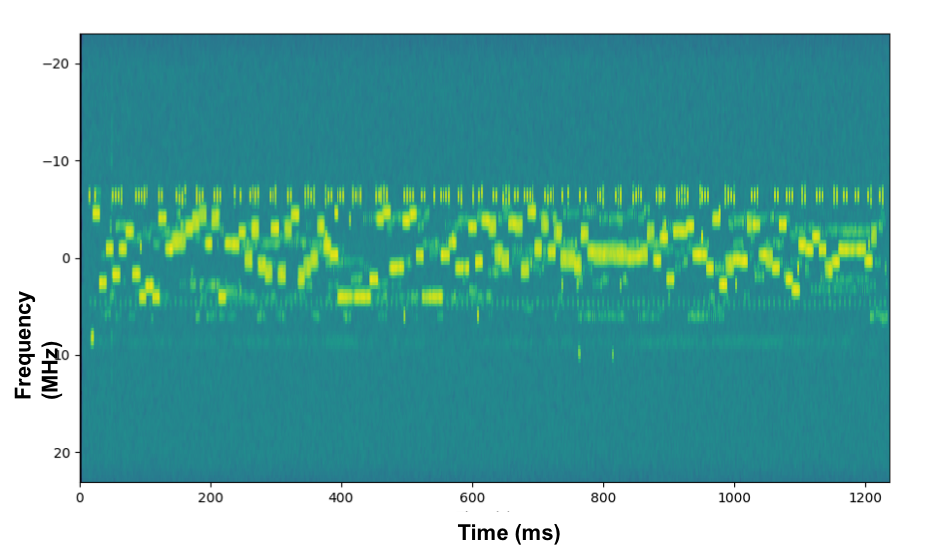
\includegraphics[width = 0.6\textwidth]{Figures/ChanAllocEx.png}}
     \caption{Occupied spectrum in an Alleys of Austin scenario \cite[Figure $9$]{func-report}.}
     \label{fig:channelalloc}
     \end{figure}
     
\subsection{Collaboration}

Although our PE2 system was not able to take full advantage of the information received through the CIL, we attempted to report as much information as we could about our state and plans to other teams. Unfortunately, our gateway did not always have access to all the details, so we had to make several approximations. For example, the number of individual mandates (IMs) that we were achieving and the duty cycle with which we were using a specific band were often inaccurate because they were computed in a distributed manner across all the nodes.

Our system did rely heavily on three CIL messages: spectrum\_usage, location\_update, and detailed\_performance. Our decision engine kept track of the latest reports from each network and used them to gauge our performance and allocate our channels. Specifically, we attempted to maximize the minimum score across the ensemble by reducing the bandwidth of our channels when we were doing well (at least two IMs above the minimum) and hoarding more bandwidth or relocating our channels entirely when we had been the worst performing for a while.

\subsection{Issues and Challenges}

During free play matches, we observed that not all nodes reported accurate GPS locations. Initially, we thought that this could be due to bugs in our peers' software, but then we realized that it is probably intended to model realistic failures in GPS reception. We therefore refined our system to detect meaningless GPS coordinates (e.g. all zeros) and replace them with a better estimate based on previously reported coordinates and those of other nodes in the same network.

\section{Results and Discussion}
We discuss our results in PE2, as well as the Payline Redux event, and highlight key aspects that will serve as guidelines for future improvements.

\subsection{Overview}
We have the following general observation from the results of our participation in PE 2 and the Payline Redux events:
\begin{enumerate}
    \item We observe that we did particularly well - in terms of scoring performance - in Slice of Life scenarios. We are working on further analyzing the logs to understand the reason, but it is likely because of the collaborative behavior that is designed to maximize the ensemble minimum and report accurate spectrum usage information.
    \item The \emph{surprise} jammer did not cause severe damage to our CIRN performance.
    \item We plan to improve our incumbent protection algorithm, as our CIRN participated in multiple matches where the incumbent threshold was violated for long periods of time.
    \item We plan to further improve our adaptive MCS algorithm, as we believe that it played a key role in not passing the payline test during PE 2. Tentative improvements led to our payline redux success, but further improvements are needed in Phase 3.
    \item We suspect that having the control channels fixed at the band edges negatively affected peer performance (as discussed in detail in Section \ref{sec:control}). We plan to improve this by adding an intelligent mechanism that backs up control updates.
    \item We plan to further add intelligent capabilities to support channel allocation, in a manner that adjusts to the current scenario and peer behavior.
\end{enumerate}
\subsection{Spectrum Reuse}

Each node is assigned a center frequency and bandwidth as described in Section~\ref{s-chan_alloc}. This is done based on the individual interference map from that node to all others in our network, allowing for spatial frequency reuse. Figure~\ref{fg:freqreuse} illustrates this behavior. However, our MAC layer does not have the capability of preventing nodes from transmitting during specific time intervals, so we were not able to take advantage of time-sharing opportunities. 

\begin{figure} [h]
 \centerline{
 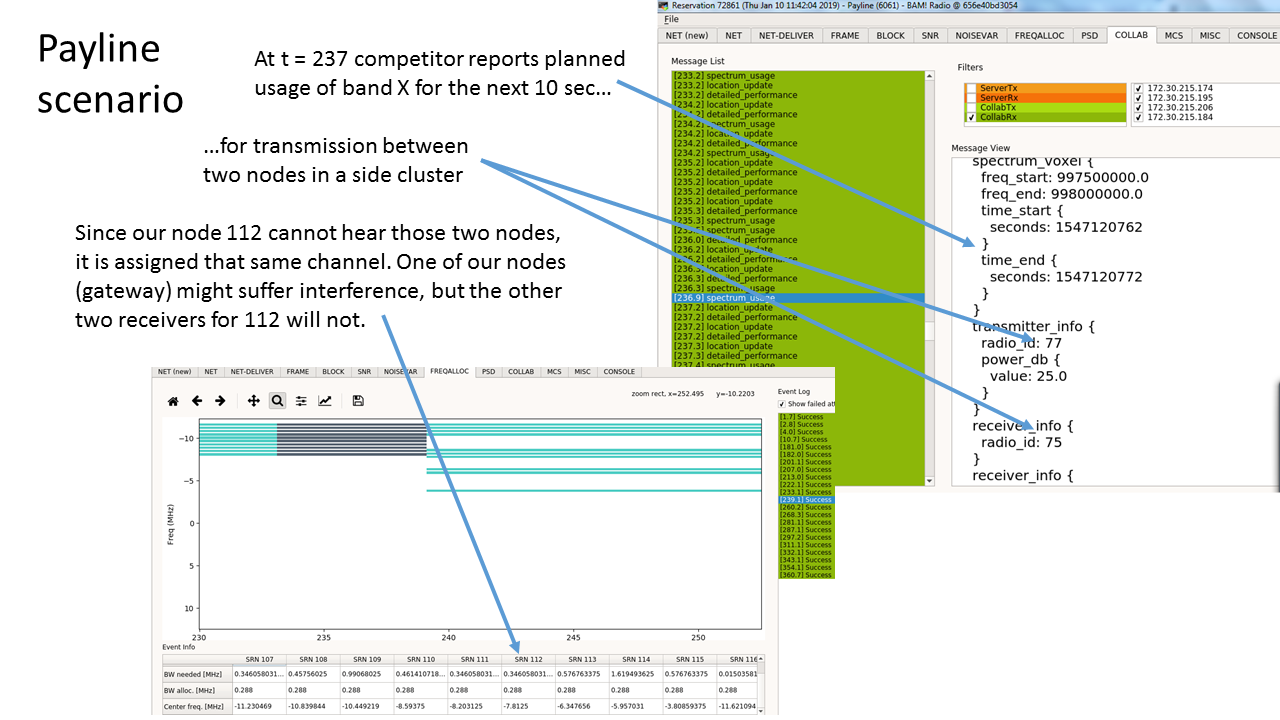
\includegraphics[width = 0.9\textwidth]{Figures/FreqReuse.png}}
 \caption{Captures from our GUI showing our spatial frequency reuse.}
 \label{fg:freqreuse}
 \end{figure} 
 
\subsection{Passive and DSRC Incumbent Protection}

We reacted in the same way for both passive and DSRC incumbents: by progressively reducing our transmit power with each violation report. Figure~\ref{fg:passiveInc} illustrates this behavior. We assumed that other teams would do the same, but might be slower than us. Therefore, we decided to stop reducing our transmit power once it had dropped 10 dB below our default transmit power (which is not the maximum allowable by the radios, since we are only using one antenna). However, we did not test this hypothesis sufficiently during free play.

From the results of the competition, it seems that our peers were not reducing their power as we were expecting, and that the tolerance threshold after a violation was lower than we expected. Therefore, our performance in the passive incumbent protection scenario was not as good as we expected.

\begin{figure} [h]
 \centerline{
 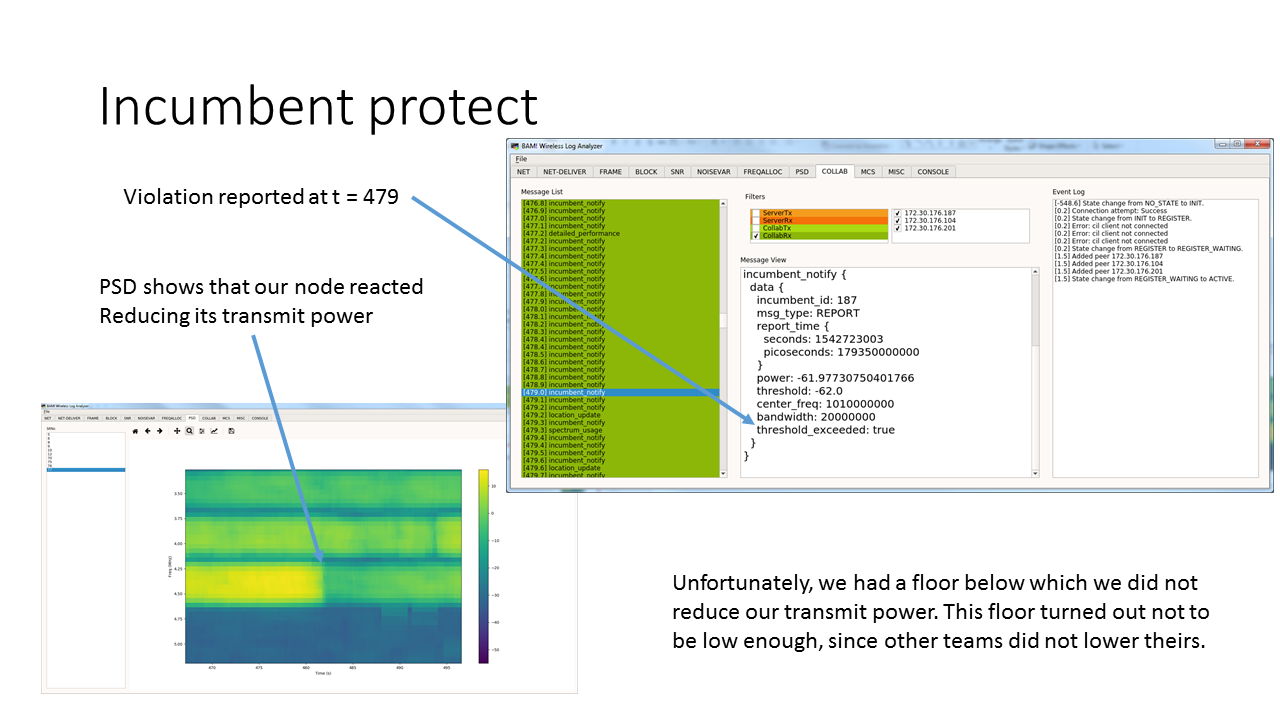
\includegraphics[width = 0.9\textwidth]{Figures/PassiveIncumbent.png}}
 \caption{Captures from our GUI showing our protection of the passive incumbent.}
 \label{fg:passiveInc}
 \end{figure} 

\subsection{Role of Collaboration}

The different roles that collaboration plays in our system have been described in most of the above sections. However, our ultimate goal in collaborative interactions was to maximize the minimum score across the ensemble at every point in time. Figure~\ref{fg:collab_chanalloc} illustrates one of the ways in which we used the CIL to achieve that goal through channel reallocation.

\begin{figure} [h]
 \centerline{
 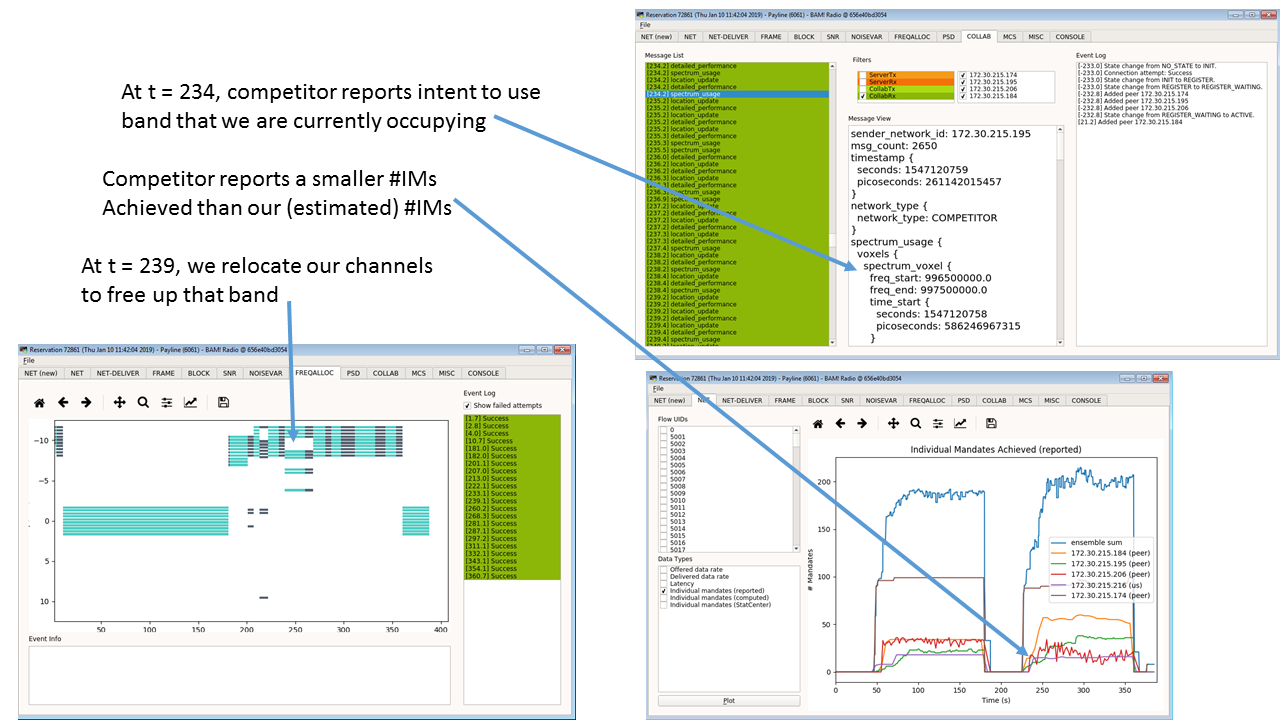
\includegraphics[width = 0.9\textwidth]{Figures/Collab_chanalloc.png}}
 \caption{Captures from our GUI showing our collaboration to maximize the minimum score across the ensemble.}
 \label{fg:collab_chanalloc}
 \end{figure}
 
\subsection{Payline Success}

We did not succeed in passing the Payline test in PE2, but were the highest ranked team that did not do so, and then successfully passed the test in the Payline Redux event. We believe that the main reasons for our initial failure was the fact that we were being excessively conservative in the adaptation of our channel bandwidths and our MCS (Modulation and Coding Scheme) was not accurately accounting for interference.

Our goal, regardless of the scenario and environment, was to maximize the minimum score across the ensemble. Whenever one of our peers reported a smaller number of IMs achieved than us, we narrowed our channels, trying to give the struggling peer the opportunity to increase their resources. This was usually the case at the beginning of each payline phase, there was always a struggling peer that we needed to help. Eventually, our number of IMs dropped, and then we widened our channels, but it was too late. Most of the bandwidth had already been claimed and the interference was too much for us to handle.

In the Payline Redux event, we changed our approach. We set a lower bound for the width of our channels. Even if others were doing badly, we would not make our channels narrower than 288 KHz. Additionally, we improved our MCS adaptation to better deal with interference.

\subsection{Issues and Challenges}

We did not pass the payline in the PE2, but did pass it in the second opportunity. We believe that our not passing the payline was in part due to the lack of opportunities to run 50 node matches in free play. Colosseum was usually too busy to schedule large jobs, so our ones would sit in the queue for very long periods. Eventually, we had to base a lot of our decisions on the results that we saw with 30 nodes, and it seems like this did not capture the case when 20 more nodes were in play. We did benefit greatly from the additional opportunity, as we could test extensively through 50 node payline reservations, and investigate the challenges that our CIRN had in the payline stage. 

\section{Conclusions}
In this paper, we provided a description of the key aspect of the BAM!\ Wireless CIRN design during Phase 2 of the DARPA Sc2 Challenge. Our current solution provides a robust and agile framework, that we can build on to add needed more sophisticated features during Phase 3. In particular, we expect that using multiple antennas and enhancing the adaptive MCS algorithm through incorporating information about the transmit power level and extensive testing, as well as noise whitening for narrowband channels would greatly enhance the physical layer. Furthermore, using non-binary routing tables as well as incorporating stream ARQ would improve the reliability of flow delivery while meeting requirements. Finally, added features in Phase 3 like the presence of active incumbents, varying scoring policies for different flows and different times of the match would also require changes to multiple parts of our design (e.g., flow scheduling and channel allocation) and added intelligent capabilities to optimize the new metrics.
\section{Recommendations}
We provide below our recommendations for the SC2 Team.
\subsection{Colosseum}
\subsubsection{Reservation Scheduling}
We recommend providing an estimate for when each pending job will be scheduled. This would greatly help us schedule our workload.
\subsubsection{Free Play Leaderboard}
We noticed that not all the reservations referenced by the circles on the leaderboard match existing reservations. We recommend fixing this issue. We also recommend showing an accumulated score and rank for each team per day, week, and month periods.
\subsection{CIRN Interaction Language}
We recommend enforcing a check for accuracy of the reported information, in particular, Spectrum Usage and Scoring Performance. The SC2 Team can also use the GPS coordinates to check for accuracy of reported locations.
\subsection{Scoring Engine}
We recommend that the SC2 Team closely interact with the CILC members who will work on developing the independent scoring engine, and provide confirmation that the developed engine provides accurate and reliable results, with respect to the one used in the competition.
\begin{thebibliography}{2}
 \bibitem{func-report}
 Team BAM!\ Wireless, ``DARPA SC2: Functioning Subsystem Design Report'', 2018.
 \end{thebibliography}
\end{document}